\documentclass[10pt, journal]{IEEEtran}
\usepackage{amsmath}
\usepackage{amsfonts}
\usepackage{amssymb}
\usepackage{hyperref}
\usepackage{graphicx}
\graphicspath{ {images/} }
\usepackage[caption=false,font=footnotesize]{subfig}

\DeclareMathOperator{\vol}{Vol}

\title{Object Detection in Scientific Images (DRAFT)}

\author{Benjamin Killeen and Gordon Kindlmann %
  \thanks{Benjamin Killeen is an undergraduate with the Department of Computer
    Science, University of Chicago, Chicago, IL 60637, USA (email:
    \href{mailto:killeen@uchicago.edu}{killeen@uchicago.edu})} %
  \thanks{Gordon Kindlmann is with the Department of Computer Science, 
    University of Chicago, Chicago, IL 60637, USA (email:
    \href{mailto:glk@uchicago.edu}{glk@uchicago.edu})} %
}

\begin{document}
\maketitle

\begin{abstract}
  Together with large training sets, Deep Neural Networks (DNNs) have enabled a
  wide range of advancements in Computer Vision tasks, especially with regard to
  object detection in real-world images. Object detection for scientific images,
  on the other hand, presents challenges unlike typical vision tasks. Scientific
  tasks exhibit \emph{governing principles} in their datasets, which result from
  the phenomena under investigation. In this progress report, we describe our
  ongoing effort toward training DNNs which are agnostic to governing principles
  yet perform reliably on scarce data.\footnote{Code available at
    \href{https://github.com/bendkill/artifice} {github.com/bendkill/artifice}}
\end{abstract}

\section{Introduction}
\label{sec:introduction}

% TODO: incorporate principle of governing principles.

% Labeling is perhaps a bad word, limiting to classification. Analysis is the
% word that we might be looking for. Real-valued multivariate descriptions of
% the values captured by those images.

Imaging systems are a vital component of many scientific experiments, used as
the primary measuring device of properties like object location or
orientation. In cases where no alternative measuring device exists, accurate
analysis is of the utmost importance. However, such image analysis can prove
labor-intensive. Traditional methods involve \emph{ad hoc} solutions suited for
one experimental setup even though more general object detection tasks have been
well-studied in Computer Vision. In this report, we introduce an ongoing effort
to generalize principles for image-data analysis across scientific tasks using
DNNs, emphasizing the importance of careful data augmentation.

% How are we saving the day?
Deep Neural Networks\footnote{Alternatively, deep convolutional neural
  networks.}  have shown remarkable success on real-world tasks
\cite{krizhevsky_imagenet_2012}, such as challenges for datasets like ImageNet
\cite{deng_imagenet:_nodate} and COCO \cite{lin_microsoft_2014}. These and other
data underlie supervised learning approaches, as in
Fig. \ref{fig:traditional-graph}, for increasingly complex tasks. Scientific
experiments, on the other hand, have no dataset except what they generate; each
experiment constitutes its own unique task, sometimes entirely disjoint from
established datasets. The man-hour investment required for labeling scientific
images motivates our approach, leveraging active learning
\cite{settles_active_2012, kao_localization-aware_2018, jain_active_2016} and
data augmentation, \cite{krizhevsky_imagenet_2012, ronneberger_u-net:_2015}. The
focus of this report, moreover, is the application of data augmentation to
reduce overfitting.             %TODO: fix this sentence.

\begin{figure*}
  \centering
  \subfloat[]{
    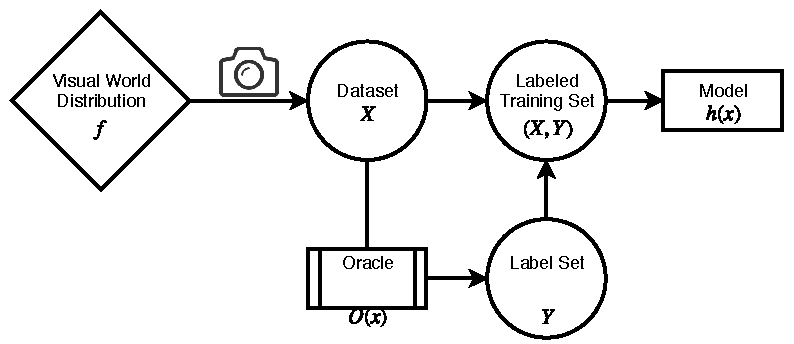
\includegraphics[width=0.46\linewidth]{traditional_graph}
    \label{fig:traditional-graph}
  }
  \hfill
  \subfloat[]{
    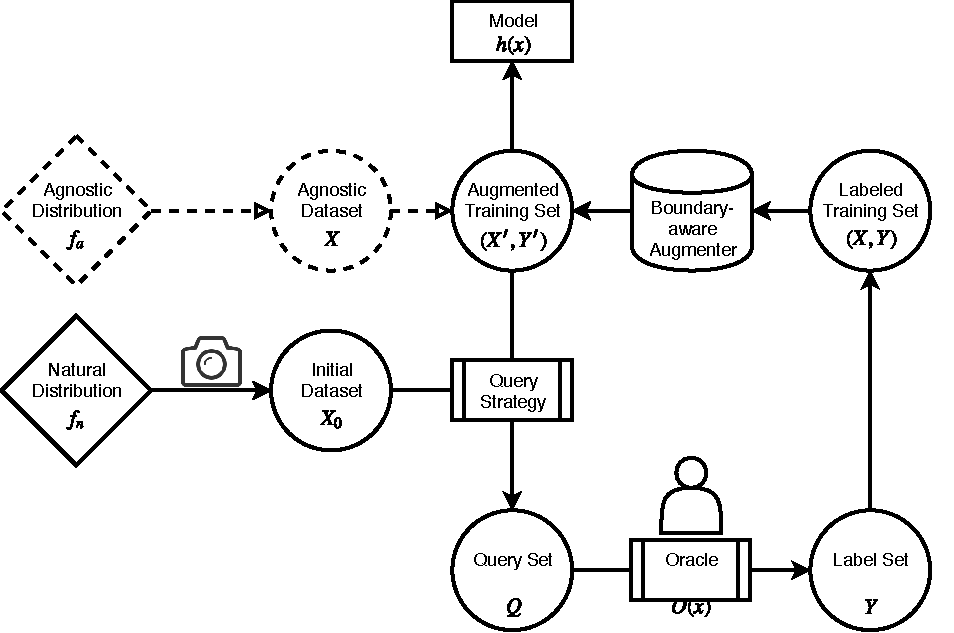
\includegraphics[width=0.50\linewidth]{artifice_graph}
    \label{fig:artifice-graph}
  }
  \caption{During supervised learning for real-world vision tasks \textbf{(a)},
    a camera samples a large dataset $X$ from the ``visual world'' distribution
    $f$. For scientific tasks \textbf{(b)}, an experiment samples a small
    initial dataset $X_0$ from the natural distribution $f_n$, which includes
    the effects of any governing principles. Our proposed training method
    incorporates a boundary-aware augmenter $A$, which uses the training set
    $(X,Y)$ to simulate drawing examples from the agnostic distribution
    $f_a$. Dashed lines indicate theoretical or simulated objects.}
  \label{fig:dependency-graphs}
\end{figure*}

\subsection{Governing Principles}
\label{sec:governing-principles}

Scientific experiments use images as a measuring technique, recovering
properties like object position or orientation for further analysis. These
quantities encode the underlying structure of the experiment, if any exists,
which is under investigation. Images of a sphere in free-fall, for example,
capture the laws of gravity, which any measurement \emph{aiming to study
  gravity} ought to ignore for the sake of scientific rigor. Experiments that
anticipate such \emph{governing principles} in the data commit a logical
fallacy by assuming the initial point. This observation is particularly
important for training DNNs in scientific tasks. Like any statistical model,
DNNS are prone to overfitting when underlying correlations are present. In order
to address this issue, we contrast scientific tasks with traditional tasks in
computer vision.

Fig. \ref{fig:traditional-graph} outlines the training process for traditional
vision tasks. Typically, such approaches leverage a large, fully labeled
training set $(X,Y)$, \textit{e.g.} ImageNet, where $X$ is the set of
$M\times N$ images and $Y\subseteq \mathbb{R}^n$ is the label set. In any task,
the labeling comprises a lower-dimensional representation of the data space,
encoding valuable information from each example. $n$ denotes the dimensionality
of the labeling, \textit{e.g.} the number of classes. Supervised learning aims
to train a model (such as a DNN)
$h : \mathbb{R}^{M\times N} \rightarrow \mathbb{R}^n$ that can interpret the
visual world. Crucial, the visual world is not a uniformly distributed set of
images; we denote its probability distribution as
$f : \mathbb{R}^{M\times N} \rightarrow \mathbb{R}$, from which every dataset
draws examples as independently and identically distributed as possible.

For real-world tasks, sampling $f$ in this manner is desirable, but in
scientific tasks, governing principles make sampling from the original
distribution impossible. In fact, for the purposes of training, we wish to
% TODO: check "impossible" wording
sample from a distribution as uniform as possible in the label space
$\mathbb{R}^n$. That is, we wish for the dataset $X$ to correspond to labels $Y$
which contain almost no structure, within reasonable boundaries. Fortunately,
most scientific experiments have well-known boundaries incorporated into their
design. A sphere in free-fall, for instance, might be bound to one-dimension by
a track, even though its image-space position is described by two
coordinates. Fig. \ref{fig:gyros} shows an experiment where dot markers are
confined to a small circular region. These \emph{label-space boundaries} are a
low-dimensional representation of a data-space region
$\chi \subseteq \mathbb{R}^{M\times N}$ such that the real distribution $f$
obeys
\[ (\forall x \not\in \chi)(f_n(x) = 0). \] Even with perfect knowledge of these
boundaries, however, it is difficult or impossible to recover $\chi$ from the
lower-dimensional label-space boundaries.
% Clarify that this is not the smallest such space, simply the smallest known.

Although $\chi$ is largely a theoretical construct, it serves as a useful
concept for training models which are agnostic to governing principles. Consider
the uniform distribution across it, which we will refer to as the \emph{agnostic
  distribution}:
\[ f_a(x) =
  \begin{cases}
    \frac{1}{\vol(\chi)} & x \in \chi \\
    0 & x \not\in \chi
  \end{cases}
\] From the initial dataset $X_0$, then, we wish to generate and label an
augmented dataset $X$ that approximates an agnostic dataset $X_a \sim f_a$. In
this report, we introduce a \emph{Boundary-Aware Augmenter} (BAA) that utilizes
label-space boundaries and instance segmentations to approach $X_a$.

\section{Related Work}
\label{sec:related-work}

% \cite{bernardis_finding_2010} uses a graph-cut approach for dot localization,
% noting various scientific applications, and \cite{ronneberger_u-net:_2015}
% applies a DNN for semantic segmentation of neuronal structures in electron
% microscope stacks.

The problems of data scarcity and biases are well-considered in computer
vision. \cite{torralba_unbiased_2011} explores bias in popular datasets for
computer vision by training DNNs on one dataset but testing them on another
(employing a test-train split for fairness). Unsurprisingly, networks perform
best on the dataset for which they were trained, even though datasets like
ImageNet aim to capture the unbiased visual world. Creating unbiased datasets
for real-world vision tasks remains an open problem, one which may demand a
reckoning for the community's focus on dataset performance scores.

\cite{ronneberger_u-net:_2015} describes a novel segmentation architecture using
up-convolutions which, paired with their data augmentation scheme, performs well
on biomedical images from electron microscope stacks. Like our approach,
\cite{ronneberger_u-net:_2015} confronts data scarcity but also focuses on
applications in biomedical imaging, where semantic segmentation is often
sufficient. We aim to address scientific tasks more generally, using semantic
segmentation as one component of a general detection system, capable of
recovering location, orientation, or shape for multiple objects. Capturing these
quantities with minimal human effort would accelerate a wide range of scientific
experiments.

% TODO: think about splitting up these figures? The reader will want to know
% what you're doing differently. Without a figure and with words alone, describe
% broadly what you're doing in the intro. Also: export to PDF and not PNG.
\begin{figure}
  \centering
  \subfloat[Gyroscopic Model]{
    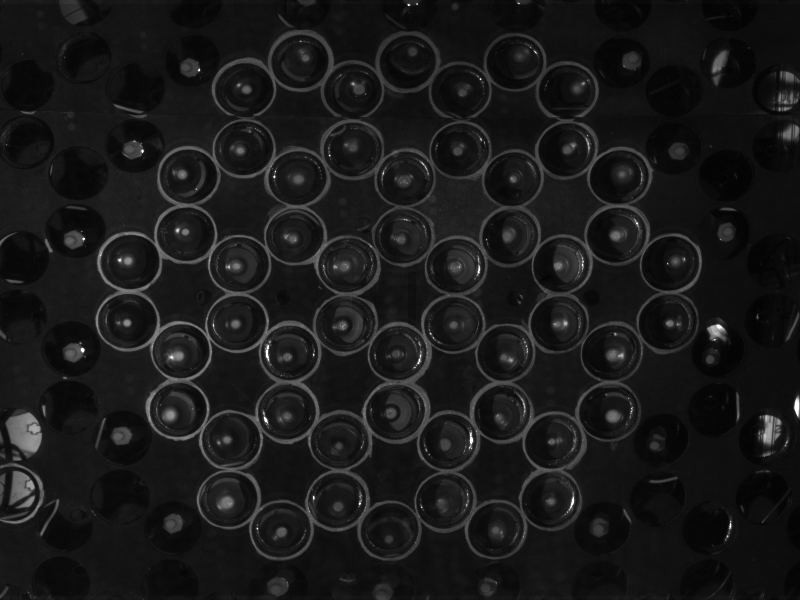
\includegraphics[height=0.37\linewidth]{gyros}
    \label{fig:gyros}
  }
  \hfill
  \subfloat[Coupled Spheres]{
    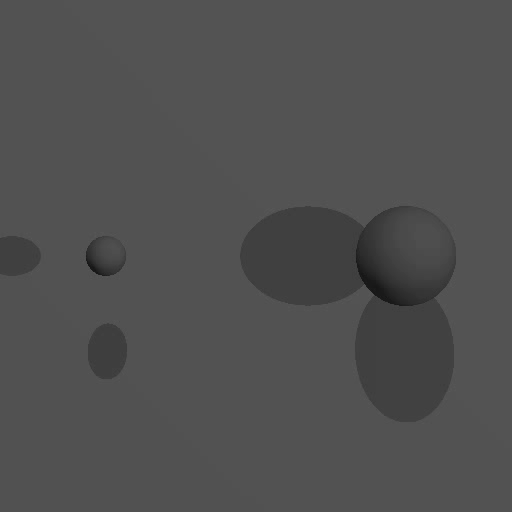
\includegraphics[height=0.37\linewidth]{coupled_spheres}
    \label{fig:coupled-spheres}
  }

  \caption[example experiments]{Example images from scientific experiments:
    \textbf{(a)} gyroscopic model for topological metamaterials
    \cite{nash_topological_2015}. Each dot is bound inside the circle
    surrounding it. \textbf{(b)} still frame from a simulated experiment of two
    spheres coupled by an invisible spring. Full video \href
    {https://github.com/bendkill/artifice/blob/master/docs/coupled_spheres.gif}
    {here}.}
  \label{fig:example-experiments}
\end{figure}

% TODO: just put citations at the end of the sentence, sentence should stand
% alone.

% TODO: not in the paper, ignoring everything, all of law's natures, in addition
% to GPs

% TODO: think about time, how are we treating the chronological ordering of the
% data?

% TODO: it's okay for the object to have some notion of continuity. The
% experimenter knows the max velocity that these things could have, puts a cap
% on the maximum distance between examples.

\section{Method}
\label{sec:method}

Our method employs a combination of active learning and data augmentation to
minimize the experimenter's labor-investment. Since this report focuses on
minimizing the effect of governing principles on the dataset, we rely on
existing literature \cite{settles_active_2012, vezhnevets_active_2012} for query
selection strategies. In spite of this, the query strategy is a vital part of
any practical application of our method, facilitating fast learning and ease of
use.

The function of the BAA is more fundamental. Like any data augmentation, scheme,
it aims to mitigate the effects of data scarcity, which
\cite{krizhevsky_imagenet_2012} achieves through image-global transformations
such as flipping and brightness shifts. In order to address governing
principles, however, the BAA must be able to generate examples $x$ from
arbitrary points $y$ in label space $\mathbb{R}^n$. In principle, the label
space can include any number of object properties which the experimenter wishes
to measure, including position in the image, apparent orientation, and
size. These apply to every object in the image, resulting in a label-space that
can grow relatively large, with independent boundary constraints for every
coordinate constraining $\chi$. For the following explanation, we consider a
label space of object positions, such for the spheres in
Fig. \ref{fig:coupled-spheres}, but maintain that the same principles apply for
higher-dimensional label spaces.

% TODO: figure illustrating segmentation augmentation?
In order to freely manipulate examples in label-space, we require an instance
segmentation of each image. With this information, we can extract the pixels
belonging to every object in the image and translate them freely. Unlike
image-global strategies, this method directly addresses the label-space
representation of an example, but it also raises two questions: what pixels
should the augmenter use to replace the extracted object, and what new points in
label-space should the augmenter introduce? The first question is a matter of
practical importance, but the second directly relates to our primary goal.

% TODO: figure illustrating inpainting?
There are many possible solutions to the problem of pixel-replacement. Most
simply, one could use the mean value of the surrounding region, or else gaussian
noise with the same mean and standard deviation. \cite{bertalmio_image_2000}
describes a more nuanced approach that attempts to complete isophote lines
arriving at the region's edge. \cite{pathak_context_2016} introduces Context
Encoders: DNNs that incorporate the entire image to inpaint a desired
region. Any of these methods should prove effective for our purposes, although
in many cases they may prove unnecessary. Many scientific tasks are the result
of fixed-camera video data. If another example in the labeled dataset includes
background pixels from the desired region, then the most effective approach
would simply ``transplant'' these pixels, so to speak, from that example.



% Because of the variety of scientific tasks, $f$ must remain flexible with regard
% to its output. Toward this end, we envision a two-step procedure which (1)
% obtains an instance segmentation \cite{ronneberger_u-net:_2015, bai_deep_2016}
% for objects of interest and (2) learns the target parameters (location,
% orientation, etc.) for each object. Whether these steps occur in an end-to-end
% fashion or are divided between several training steps is an open question. We
% do, however, consider (1) to be a vital step for the sake of maintaining
% generality. Even in scientific tasks where segmentation is unneeded, such as the
% Coupled Sphere experiment in \ref{sec:method}, obtaining pixel-level masks of
% each object enables more advanced data augmentation methods.

% Because we wish to minimize the man-hours required for training as much as
% possible, we use an active learning scheme to select a query set
% $Q \subseteq X'$ which will most inform training. The application of active
% learning to semantic segmentation has received relatively little attention, with
% the exception of \cite{vezhnevets_active_2012}, and the added complication of an
% imperfect labeler remains an open question in the field
% \cite{settles_active_2012}. We aim to address both issues with its
% \emph{selector}.

% Finally, the \emph{augmenter} will incorporate both the semantic segmentations
% obtained by $f$ and the imposed constraints specified by the experimenter to
% improve training as much as possible. We hope to test many augmentation methods
% while keeping in mind that the image space of a scientific task is usually much
% more constrained than that of a real-world
% task. \cite{krizhevsky_imagenet_2012}, for instance, uses sub-image extraction,
% flipping, and PCA analysis of RGB channels to augment ImageNet. These methods
% are not necessarily applicable to scientific tasks, where imposed constraints
% might invalidate a flipped image, for instance.

\section{Simulated Experiments}
\label{sec:simulated-experiments}

TODO: UPDATE SIMULATED EXPERIMENTS

In order to show our method's effectiveness, we develop several virtual
experiments. These simulations offer several advantages over images from real
experiments, such as in Fig. \ref{fig:gyros}. First, we have perfect knowledge
of the experiment's ``Truth'' $\tilde{Y}$, as opposed to imperfect measurements,
or ``ground truth,'' $Y$. In well established datasets, $\tilde{Y}$ and $Y$ are
nearly identical, but we must rely on one or a few human labelers for what
should be unambiguous quantities. For testing, we calculate $\tilde{Y}$ from the
known parameters of the simulation, and we emulate a human labeler by
introducing small perturbations to $\tilde{Y}$, producing $Y$. Part of
our goal is to train a DNN with predictions $\hat{Y}$ that more closely
approximate $\tilde{Y}$ than the labels $Y$. Simulated experiments allow us to
test this performance.

Fig. \ref{fig:coupled-spheres} shows one such experiment. In this case, two
spheres with different masses rotate in free space, coupled by an invisible
spring. The goal of the Coupled Spheres experiment is to recover physical
properties of the spring using $(x,y)$ positions of the two spheres. Imposed
constraints include the $z$-coordinate of each sphere, which is set to the
image-plane, as well as each sphere's apparent size. Inherent constraints
include the physical properties of the spring, \textit{e.g.} the spring constant
and relaxed length. Adverse noise, which in this case includes any shadows,
lighting effects, and possible occlusion, also presents a challenge for
detection.

To demonstrate our method's resilience to inherent constraints, we intend to
train a DNN on one experiment and evaluate its performance on experiments with
different simulated springs. This simple example illustrates the general
resilience that we wish to develop.

\section{Conclusion}
\label{sec:conclusion}

TODO: CONCLUSION

\section*{Acknowledgment}
\label{sec:acknowledgment}

Thanks to Michael Maire for input and guidance, as well as William Irvine for
access to image data from his laboratory.

\bibliographystyle{IEEEtran}
\bibliography{IEEEabrv, report}

\end{document}
%%% Local Variables:
%%% mode: latex
%%% TeX-master: t
%%% End:
